\documentclass[12pt,a4paper]{report}

% Packages
\usepackage[utf8]{inputenc}
\usepackage[T1]{fontenc}
\usepackage[french,english]{babel}
\usepackage{geometry}
\usepackage{amsmath,amsfonts,amssymb}
\usepackage{graphicx,rotating}
\usepackage{float}
\usepackage{caption}
\usepackage{subcaption}
\usepackage{listings}
\usepackage{xcolor}
\usepackage{hyperref}
\usepackage{fancyhdr}
\usepackage{titlesec}
\usepackage{tocloft}
\usepackage{acronym}
\usepackage{booktabs}
\usepackage{longtable}
\usepackage{array}
\usepackage{wrapfig}
\usepackage{multirow}
\usepackage{tikz}
\usepackage{pgfplots}
\usepackage{minted}
\usepackage{appendix}
\usepackage{svg}

% Page geometry
\geometry{
    left=1cm,
    right=1cm,
    top=2.5cm,
    bottom=2.5cm
}

% Line spacing
\usepackage{setspace}
\onehalfspacing

% Headers and footers
\pagestyle{fancy}
\fancyhf{}
\fancyhead[L]{\leftmark}
\fancyhead[R]{\thepage}
\renewcommand{\headrulewidth}{0.4pt}

% Hyperref setup
\hypersetup{
    colorlinks=true,
    linkcolor=blue,
    filecolor=magenta,
    urlcolor=cyan,
    citecolor=red,
    pdftitle={Financial Data Surveillance System - Internship Report},
    pdfauthor={[Your Name]},
    pdfsubject={Internship Report},
    pdfkeywords={Financial Data, Real-time Processing, Anomaly Detection}
}

% Code listing setup
\lstset{
    backgroundcolor=\color{gray!10},
    basicstyle=\ttfamily\small,
    breaklines=true,
    captionpos=b,
    commentstyle=\color{green!60!black},
    keywordstyle=\color{blue},
    stringstyle=\color{red},
    numberstyle=\tiny\color{gray},
    numbers=left,
    frame=single,
    rulecolor=\color{black!30},
    showstringspaces=false,
    tabsize=2
}

% Python syntax highlighting
\lstdefinestyle{python}{
    language=Python,
    morekeywords={self,def,class,if,else,elif,while,for,in,return,import,from,as,try,except,finally,with,yield,lambda}
}

% Custom commands
\newcommand{\code}[1]{\texttt{#1}}
\newcommand{\file}[1]{\texttt{#1}}
\newcommand{\keyword}[1]{\textbf{#1}}

\begin{document}

% Include all chapters
% % Cover Page
\begin{titlepage}
    \centering
    
    % University/Institution logo (if available)
    % \includegraphics[width=0.3\textwidth]{figures/university_logo.png}\\[1cm]
    
    {\LARGE \textbf{[Your University/Institution Name]} \par}
    \vspace{0.5cm}
    {\large Department of Computer Science / Engineering \par}
    
    \vspace{2cm}
    
    {\Huge \textbf{INTERNSHIP REPORT} \par}
    \vspace{1cm}
    
    {\LARGE \textbf{Financial Data Surveillance System} \par}
    \vspace{0.5cm}
    {\large Real-time Anomaly Detection and Alert System \par}
    
    \vspace{2cm}
    
    % Student information
    \begin{tabular}{ll}
        \textbf{Student:} & [Your Full Name] \\[0.3cm]
        \textbf{Student ID:} & [Your Student ID] \\[0.3cm]
        \textbf{Program:} & [Your Program/Degree] \\[0.3cm]
        \textbf{Academic Year:} & 2024-2025 \\[0.3cm]
    \end{tabular}
    
    \vspace{1.5cm}
    
    % Internship information
    \begin{tabular}{ll}
        \textbf{Host Company:} & [Company Name] \\[0.3cm]
        \textbf{Internship Period:} & [Start Date] - [End Date] \\[0.3cm]
        \textbf{Duration:} & [X months] \\[0.3cm]
    \end{tabular}
    
    \vspace{1.5cm}
    
    % Supervisors
    \begin{tabular}{ll}
        \textbf{Academic Supervisor:} & [Prof. Name] \\[0.3cm]
        \textbf{Professional Supervisor:} & [Supervisor Name] \\[0.3cm]
        \textbf{Defense Date:} & [Defense Date] \\[0.3cm]
    \end{tabular}
    
    \vfill
    
    {\large \today \par}
    
\end{titlepage}

% Reset page numbering after title page
\pagenumbering{roman}
\setcounter{page}{1}

% Table of Contents
\tableofcontents
\newpage

% List of Figures
\listoffigures
\newpage

% List of Tables
\listoftables
\newpage

% List of Code Listings
\lstlistoflistings
\newpage

% Acronyms and Abbreviations
\chapter*{List of Acronyms and Abbreviations}
\addcontentsline{toc}{chapter}{List of Acronyms and Abbreviations}

\begin{acronym}
    \acro{API}{Application Programming Interface}
    \acro{CSV}{Comma-Separated Values}
    \acro{CPU}{Central Processing Unit}
    \acro{JSON}{JavaScript Object Notation}
    \acro{JWT}{JSON Web Token}
    \acro{PDF}{Portable Document Format}
    \acro{REST}{REpresentational State Transfer}
    \acro{SQL}{Structured Query Language}
    \acro{UI}{User Interface}
    \acro{URL}{Uniform Resource Locator}
    \acro{AWS}{Amazon Web Services}
    \acro{ML}{Machine Learning}
    \acro{IoT}{Internet of Things}
    \acro{TCP}{Transmission Control Protocol}
    \acro{HTTP}{HyperText Transfer Protocol}
    \acro{HTTPS}{HyperText Transfer Protocol Secure}
    \acro{SSL}{Secure Sockets Layer}
    \acro{TLS}{Transport Layer Security}
    \acro{RAM}{Random Access Memory}
    \acro{SSD}{Solid State Drive}
    \acro{HDD}{Hard Disk Drive}
    \acro{IDE}{Integrated Development Environment}
    \acro{CI/CD}{Continuous Integration/Continuous Deployment}
    \acro{DevOps}{Development Operations}
    \acro{TSLA}{Tesla Inc. Stock Symbol}
    \acro{AAPL}{Apple Inc. Stock Symbol}
    \acro{NYSE}{New York Stock Exchange}
    \acro{NASDAQ}{National Association of Securities Dealers Automated Quotations}
\end{acronym}

\newpage

% Reset page numbering for main content
\pagenumbering{arabic}
\setcounter{page}{1}

% Chapter 1: Introduction
\chapter{Introduction}

\section{General Context}

The financial markets operate in an increasingly complex and volatile environment where price movements can occur within microseconds. The importance of real-time financial surveillance has grown exponentially with the rise of algorithmic trading, high-frequency trading, and the democratization of financial markets through retail trading platforms.

Modern financial institutions and regulatory bodies require sophisticated systems capable of monitoring thousands of financial instruments simultaneously, detecting anomalous price movements, and generating alerts in real-time. These systems must process massive volumes of data while maintaining low latency and high accuracy to prevent market manipulation, detect insider trading, and ensure market integrity.

The evolution of data processing technologies, particularly in the areas of stream processing, distributed computing, and machine learning, has opened new possibilities for creating more efficient and accurate surveillance systems. Technologies such as Apache Kafka for real-time data streaming, Elasticsearch for fast search and analytics, and modern frameworks like FastAPI for building high-performance APIs have revolutionized how financial data can be processed and analyzed.

\section{Problem Statement}

Financial markets generate enormous amounts of data every second, with price updates, trading volumes, and market events occurring continuously across multiple exchanges and trading venues. Traditional surveillance systems often struggle with several key challenges:
% % Cover Page
\begin{titlepage}
    \centering
    
    % University/Institution logo (if available)
    % \includegraphics[width=0.3\textwidth]{figures/university_logo.png}\\[1cm]
    
    {\LARGE \textbf{[Your University/Institution Name]} \par}
    \vspace{0.5cm}
    {\large Department of Computer Science / Engineering \par}
    
    \vspace{2cm}
    
    {\Huge \textbf{INTERNSHIP REPORT} \par}
    \vspace{1cm}
    
    {\LARGE \textbf{Financial Data Surveillance System} \par}
    \vspace{0.5cm}
    {\large Real-time Anomaly Detection and Alert System \par}
    
    \vspace{2cm}
    
    % Student information
    \begin{tabular}{ll}
        \textbf{Student:} & [Your Full Name] \\[0.3cm]
        \textbf{Student ID:} & [Your Student ID] \\[0.3cm]
        \textbf{Program:} & [Your Program/Degree] \\[0.3cm]
        \textbf{Academic Year:} & 2024-2025 \\[0.3cm]
    \end{tabular}
    
    \vspace{1.5cm}
    
    % Internship information
    \begin{tabular}{ll}
        \textbf{Host Company:} & [Company Name] \\[0.3cm]
        \textbf{Internship Period:} & [Start Date] - [End Date] \\[0.3cm]
        \textbf{Duration:} & [X months] \\[0.3cm]
    \end{tabular}
    
    \vspace{1.5cm}
    
    % Supervisors
    \begin{tabular}{ll}
        \textbf{Academic Supervisor:} & [Prof. Name] \\[0.3cm]
        \textbf{Professional Supervisor:} & [Supervisor Name] \\[0.3cm]
        \textbf{Defense Date:} & [Defense Date] \\[0.3cm]
    \end{tabular}
    
    \vfill
    
    {\large \today \par}
    
\end{titlepage}

% Reset page numbering after title page
\pagenumbering{roman}
\setcounter{page}{1}

\begin{itemize}
    \item \textbf{Real-time Processing}: The need to process and analyze financial data in real-time to detect anomalies as they occur, rather than discovering them hours or days later.
    
    \item \textbf{Scalability}: The ability to handle increasing volumes of data as more financial instruments are monitored and as market activity grows.
        
    \item \textbf{Historical Analysis}: Maintaining comprehensive historical records for post-mortem analysis, regulatory compliance, and pattern recognition.
    
    \item \textbf{Alert Management}: Providing timely and actionable alerts to the appropriate stakeholders when anomalies are detected.
\end{itemize}

The challenge lies in building a system that can address all these requirements simultaneously while remaining cost-effective and maintainable.
\section{Requirements}

To address the challenges outlined in the problem statement, the proposed system must satisfy a set of functional and non-functional requirements.

\subsection{Functional Requirements}
Functional requirements define the specific behaviors and capabilities of the system. For this financial surveillance system, these include:
\begin{itemize}
    \item \textbf{Data Ingestion}: The system must be able to ingest real-time financial data from various sources, including market data feeds and trading platforms.
    \item \textbf{Anomaly Detection}: The system must implement algorithms to detect various types of anomalies, such as unusual price movements, abnormal trading volumes, and deviations from historical patterns.
    \item \textbf{Alerting Mechanism}: Upon detection of an anomaly, the system must generate and deliver timely alerts to designated users or systems through multiple channels (e.g., via Kafka topics, Email, ...).
    \item \textbf{Data Storage and Retrieval}: The system must store historical financial data and detected anomalies for auditing, reporting, and further analysis. It should provide efficient mechanisms for data retrieval.
    \item \textbf{API Interface}: The system should provide a well-documented API interface to allow integration with external systems for configuration, monitoring, alert retrieval, and report generation.
    \item \textbf{Reporting}: The system should be capable of generating customizable reports summarizing detected anomalies, system performance, and market trends.
\end{itemize}

\subsection{Non-Functional Requirements}
Non-functional requirements define the quality attributes of the system. Key non-functional requirements for this project include:
\begin{itemize}
    \item \textbf{Performance}: The system must process data and detect anomalies with low latency, typically within sub-second timeframes, to be effective in real-time markets.
    \item \textbf{Scalability}: The system architecture must be scalable to handle increasing volumes of data, a growing number of monitored financial instruments, and an expanding user base without degradation in performance.
    \item \textbf{Reliability and Availability}: The system must be highly reliable and available, minimizing downtime to ensure continuous market surveillance. This includes fault tolerance and data redundancy.
    \item \textbf{Accuracy}: The anomaly detection algorithms must achieve a high level of accuracy, minimizing both false positives (incorrectly identifying normal behavior as anomalous) and false negatives (failing to detect actual anomalies).
    \item \textbf{Security}: The system must ensure the confidentiality, integrity, and availability of sensitive financial data. This includes secure data transmission, storage, and access controls.
    \item \textbf{Maintainability}: The system should be designed in a modular and well-documented manner to facilitate easy maintenance, updates, and future enhancements.
\end{itemize}


% \section{Adopted Methodology}

% The development of this financial surveillance system follows a structured approach that emphasizes iterative development, open-source technologies, and comprehensive testing:

% \subsection{Open-Source Technology Preference}

% Priority is given to open-source technologies to ensure cost-effectiveness, community support, and avoid vendor lock-in. The selected technology stack includes:
% \begin{itemize}
%     \item Apache Kafka for real-time data streaming
%     \item Elasticsearch for data storage and search
%     \item FastAPI for RESTful API development
%     \item Redis for caching and temporary data storage
%     \item Celery for asynchronous task processing
% \end{itemize}

% \subsection{Data-Driven Testing Strategy}

% The system is tested using both simulated and real financial data to ensure robustness and accuracy. Initial testing uses controlled, simulated datasets to validate core functionality, followed by testing with real market data to verify performance under actual conditions.

% \subsection{Microservices Architecture}

% The system is designed using a microservices architecture to ensure modularity, scalability, and maintainability. Each component has a specific responsibility and can be developed, tested, and deployed independently.

\section{Report Structure}

This report is organized into three main chapters, each focusing on a specific aspect of the project:
\begin{itemize}
    \item \textbf{Chapter 1} introduces the project, presenting the general context, problem statement, and requirements.
    
    \item \textbf{Chapter 2} describes the actual work, including the system design, architectural choices, implementation details, and the decisions made throughout the project.
    
    \item \textbf{Chapter 3} concludes the report, summarizing the main achievements, lessons learned, and providing perspectives for future development.
\end{itemize}

% Chapter 3: Design and Architecture


\chapter{Design and Architecture}


\section{Global System Architecture}

\subsection{Overview}

The financial data surveillance system is designed as a distributed, event-driven architecture composed of several interconnected microservices. This architecture ensures scalability, resilience, and maintainability, which are critical for real-time financial applications.

\begin{figure}[H]
    \centering
    % Placeholder for the general architecture diagram
    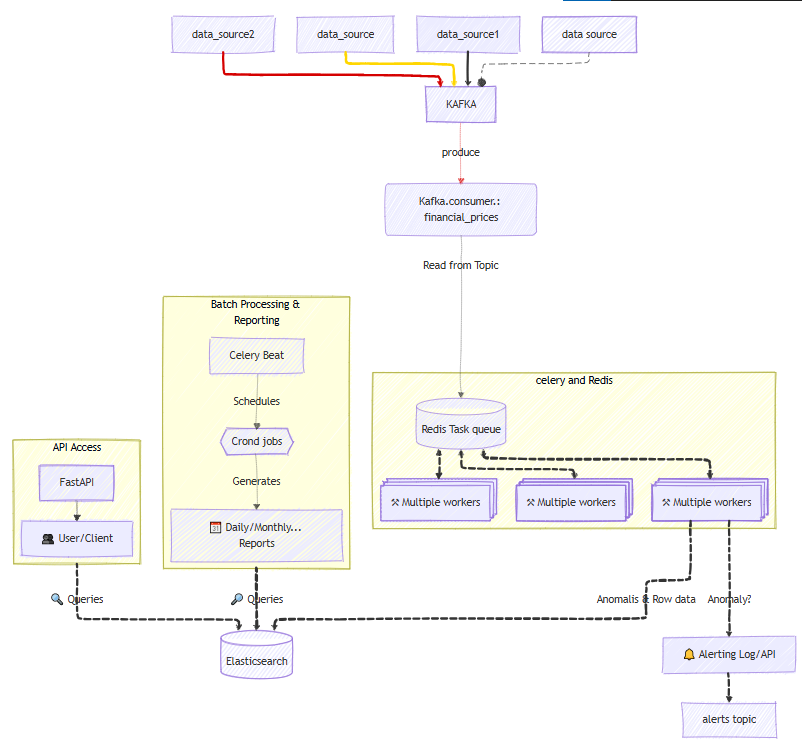
\includegraphics[width=\textwidth]{figures/global.png}
    % \fbox{\parbox[c][10cm][c]{\textwidth}{\centering Placeholder for General Architecture Diagram (e.g., using TikZ or an imported image)}}
    % \caption{General System Architecture}
    % \label{fig:general_architecture}
\end{figure}

\textbf{Main Data Flow:}
\begin{enumerate}
    \item \textbf{Data Ingestion}: Simulated financial data (e.g., TSLA stock prices) is generated and published to an Apache Kafka topic.
    \item \textbf{Real-time Processing}: Kafka consumers read data streams, and Celery workers process these messages asynchronously to detect anomalies using the Z-score algorithm. Redis is used for storing sliding windows of recent data for calculations.
    \item \textbf{Anomaly Storage}: Detected anomalies are indexed and stored in Elasticsearch for historical analysis and querying.
    \item \textbf{API and Reporting}: A FastAPI application provides RESTful endpoints for querying anomalies, generating reports (PDF, CSV), and managing alerts. Alerts are also published to separate Kafka topics for consumption by notification services.
\end{enumerate}

\textbf{Components and Their Interactions:}
\begin{itemize}
    \item \textbf{Data Generator}: Produces simulated stock price data.
    \item \textbf{Kafka Cluster}: Acts as the central message bus for data streams and alerts.
    \item \textbf{Celery Workers}: Perform asynchronous anomaly detection tasks.
    \item \textbf{Redis}: Provides fast, in-memory storage for sliding windows.
    \item \textbf{Elasticsearch Cluster}: Stores and indexes detected anomalies for long-term analysis.
    \item \textbf{FastAPI Application}: Exposes system functionalities through a REST API.
    \item \textbf{Reporting Module}: Generates analytical reports.
    \item \textbf{Alerting System}: Manages and dispatches alerts.
\end{itemize}

\subsection{Architectural Pattern}

\subsubsection{Microservices Architecture}

The choice of a microservices architecture is justified by:
\begin{itemize}
    \item \textbf{Scalability}: Individual services can be scaled independently based on demand (e.g., scaling Celery workers during high data load).
    \item \textbf{Resilience}: Failure in one service does not necessarily bring down the entire system. For instance, if the reporting service fails, data ingestion and anomaly detection can continue.
    \item \textbf{Technology Diversity}: Different services can be implemented using the most suitable technology stack for their specific tasks.
    \item \textbf{Maintainability}: Smaller, focused services are easier to understand, develop, test, and maintain.
    \item \textbf{Independent Deployability}: Services can be deployed and updated independently, allowing for faster release cycles.
\end{itemize}

\subsubsection{Event-Driven Architecture (EDA)}

An event-driven architecture, primarily facilitated by Apache Kafka, offers several advantages:
\begin{itemize}
    \item \textbf{Decoupling}: Producers and consumers of data are decoupled. The data generator does not need to know about the anomaly detection workers, and vice-versa.
    \item \textbf{Asynchronous Processing}: Tasks like anomaly detection can be performed asynchronously, improving system responsiveness and throughput.
    \item \textbf{Scalability and Resilience}: Kafka itself is highly scalable and fault-tolerant, contributing to the overall system's robustness.
    \item \textbf{Real-time Capabilities}: EDA is well-suited for real-time applications where immediate response to events (like new price data) is crucial.
\end{itemize}

\subsubsection{Separation of Concerns}

Each layer and component in the architecture has a distinct responsibility:
\begin{itemize}
    \item \textbf{Data Collection Layer}: Focuses solely on ingesting and formatting raw data.
    \item \textbf{Processing Layer}: Handles the core logic of anomaly detection.
    \item \textbf{Storage Layer}: Manages persistent storage and indexing of anomalies.
    \item \textbf{API and Reporting Layer}: Provides interfaces for user interaction and data retrieval.
\end{itemize}
This separation simplifies development, testing, and maintenance.

\section{Technology Overview and Selection Rationale}

The implementation of this system relies on several key technologies, each chosen for specific capabilities they bring to the architecture. This section provides a focused explanation of each core technology and its role in the system.

\subsection{Apache Kafka}

\subsubsection{Overview}


\begin{wrapfigure}{l}{2.5cm}  % 'l' = left side, 2.5cm = width of the box
    \vspace{-10pt} % Adjust vertical spacing
    
\includegraphics[width=2.3cm]{figures/0_CuYxguE1vG7PLngW.png}
    \vspace{-10pt}
\end{wrapfigure}

Apache Kafka is a distributed event streaming platform used in our architecture for real-time data ingestion and message propagation. It provides a highly reliable, scalable system for publishing and subscribing to streams of records.



\subsubsection{Core Features}
\begin{itemize}
    \item \textbf{Distributed Architecture}: Kafka operates as a cluster of broker nodes, providing fault tolerance and load distribution.
    \item \textbf{Topic-Based Messaging}: Data streams are organized into topics that can be partitioned for parallel processing.
    \item \textbf{High Throughput}: Capable of handling millions of messages per second with minimal latency.
    \item \textbf{Persistent Storage}: Messages are persisted to disk with configurable retention periods.
    \item \textbf{Replication}: Data is replicated across multiple nodes to prevent data loss.
\end{itemize}

\subsubsection{Kafka Architecture}

\begin{figure}[H]
    \centering
    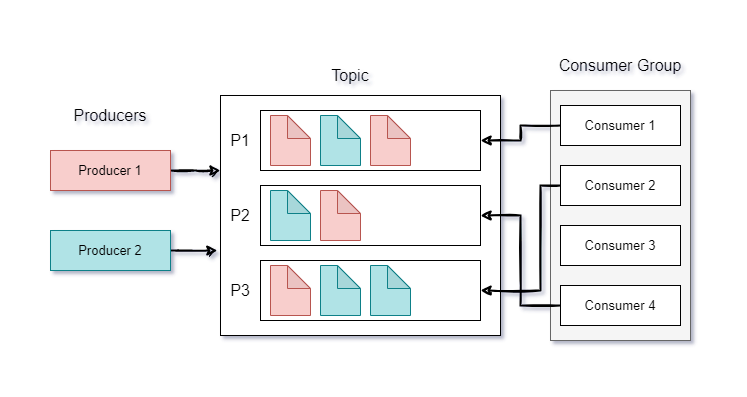
\includegraphics[width=0.75\textwidth]{figures/kafka.png}
    \caption{Kafka Architecture}
    \label{fig:kafka_architecture}
\end{figure}

\subsubsection{Role in Our System}
In our financial surveillance system, Kafka serves as:
\begin{itemize}
    \item The central data highway for stock price data streams
    \item A buffer system that decouples data producers from consumers
    \item A scalable mechanism for distributing data to multiple processing workers
    \item An event bus for propagating detected anomalies to notification services
\end{itemize}

\subsection{Redis}

\subsubsection{Overview}


\begin{wrapfigure}{l}{2.5cm}  % 'l' = left side, 2.5cm = width of the box
    \vspace{-10pt} % Adjust vertical spacing
    
\includegraphics[width=2.3cm]{figures/redis.png}
    \vspace{-10pt}
\end{wrapfigure}



Redis is an in-memory data structure store that we use both as a message broker for Celery and for maintaining sliding windows of recent stock data.

\subsubsection{Core Features}
\begin{itemize}
    \item \textbf{In-Memory Operation}: Extremely fast read/write operations with sub-millisecond latency.
    \item \textbf{Data Structures}: Supports various data structures like strings, hashes, lists, sets, and sorted sets.
    \item \textbf{Optional Persistence}: Can persist data to disk through snapshotting or append-only files.
    \item \textbf{Atomic Operations}: Supports transactions and Lua scripting for complex operations.
    \item \textbf{Pub/Sub Capabilities}: Native support for publish/subscribe messaging patterns.
\end{itemize}

\subsubsection{Role in Our System}
Redis performs two critical functions:
\begin{itemize}
    \item \textbf{Sliding Window Management}: Stores recent price data points for calculating moving statistics (mean, standard deviation) with extremely low latency.
    \item \textbf{Celery Broker}: Acts as the message broker for Celery, queuing anomaly detection tasks.
\end{itemize}

\subsection{Celery}

\subsubsection{Overview}


\begin{wrapfigure}{l}{2.5cm}  % 'l' = left side, 2.5cm = width of the box
    \vspace{-10pt} % Adjust vertical spacing
    
\includegraphics[width=2.3cm]{figures/Celery_logo.png}
    \vspace{-10pt}
\end{wrapfigure}



Celery is an asynchronous task queue/job system based on distributed message passing. It handles the background processing of anomaly detection in our architecture.

\subsubsection{Core Features}
\begin{itemize}
    \item \textbf{Asynchronous Task Execution}: Allows non-blocking execution of CPU-intensive or I/O-bound tasks.
    \item \textbf{Task Scheduling}: Supports both immediate and scheduled task execution.
    \item \textbf{Worker Pools}: Tasks can be distributed across multiple worker processes or machines.
    \item \textbf{Result Storage}: Task results can be stored and retrieved asynchronously.
    \item \textbf{Monitoring}: Tools like Flower provide real-time monitoring of task execution.
\end{itemize}

\subsubsection{Role in Our System}
Celery manages:
\begin{itemize}
    \item Asynchronous execution of anomaly detection algorithms
    \item Distribution of processing load across multiple worker instances
    \item Reliable task execution with automatic retries for failed tasks
\end{itemize}

\subsection{Elasticsearch}



\subsubsection{Overview}


\begin{wrapfigure}{l}{2.5cm}  % 'l' = left side, 2.5cm = width of the box
    \vspace{-10pt} % Adjust vertical spacing
    
\includegraphics[width=2.3cm]{figures/Elasticsearhc.png}
    \vspace{-10pt}
\end{wrapfigure}



Elasticsearch is a distributed, RESTful search and analytics engine used for storing and querying detected anomalies.

\subsubsection{Core Features}
\begin{itemize}
    \item \textbf{Document-Oriented}: Stores data as JSON documents with flexible schema.
    \item \textbf{Full-Text Search}: Powerful search capabilities with relevance scoring.
    \item \textbf{Analytics}: Built-in aggregation framework for data analytics.
    \item \textbf{Distributed Architecture}: Scales horizontally across multiple nodes.
    \item \textbf{Real-Time Operations}: Near real-time indexing and search capabilities.
\end{itemize}

\subsubsection{Role in Our System}
Elasticsearch serves as:
\begin{itemize}
    \item The persistent storage for detected anomalies
    \item A search engine for querying historical anomalies by various parameters (time range, symbol, severity)
    \item An analytics platform for trend analysis and reporting on anomalies
\end{itemize}

\subsection{FastAPI}

\subsubsection{Overview}

\begin{wrapfigure}{l}{2.5cm}  % 'l' = left side, 2.5cm = width of the box
    \vspace{-10pt} % Adjust vertical spacing
    
\includegraphics[width=2.3cm]{figures/FastAPI_logo.png}
    \vspace{-10pt}
\end{wrapfigure}


FastAPI is a modern, high-performance web framework for building APIs with Python, based on standard Python type hints.

\subsubsection{Core Features}
\begin{itemize}
    \item \textbf{Performance}: One of the fastest Python frameworks available, comparable to NodeJS and Go.
    \item \textbf{Automatic Documentation}: Generates interactive API documentation from code.
    \item \textbf{Data Validation}: Built-in request validation using Pydantic models.
    \item \textbf{Asynchronous Support}: Native support for async/await syntax.
    \item \textbf{Standards-Based}: Based on open standards like OpenAPI and JSON Schema.
\end{itemize}

\subsubsection{Role in Our System}
FastAPI provides:
\begin{itemize}
    \item RESTful endpoints for querying anomalies and generating reports
    \item A user-friendly API for interacting with the surveillance system
    \item Authentication and authorization for secure access to sensitive financial data
    \item Input validation for all API requests
\end{itemize}


\subsection{Docker}

\subsubsection{Overview}

\begin{wrapfigure}{l}{2.5cm}
    \vspace{-10pt}
    \includegraphics[width=2.3cm]{figures/docker.png}
    \vspace{-10pt}
\end{wrapfigure}

Docker is a platform for developing, shipping, and running applications in lightweight, portable containers. It enables consistent environments across development, testing, and production.

\subsubsection{Core Features}
\begin{itemize}
    \item \textbf{Containerization}: Packages applications and dependencies into isolated containers.
    \item \textbf{Portability}: Ensures applications run the same way on any system with Docker installed.
    \item \textbf{Resource Efficiency}: Containers share the host OS kernel, reducing overhead compared to virtual machines.
    \item \textbf{Rapid Deployment}: Containers can be started, stopped, and replicated quickly.
    \item \textbf{Ecosystem}: Rich tooling (Docker Compose, Docker Hub) and integration with CI/CD pipelines.
\end{itemize}

\subsubsection{Role in Our System}
Docker is used to:
\begin{itemize}
    \item Containerize all core services (Kafka, Redis, Elasticsearch, etc.) for reproducible deployments.
    \item Simplify orchestration and networking using Docker Compose.
    \item Enable easy scaling and management of microservices.
    \item Provide isolated, consistent environments for development and production.
\end{itemize}

\section{Detailed Components}

\subsection{Data Collection Layer}

\subsubsection{Data Generator}

A Python script simulates real-time stock price data for a specific symbol (e.g., TSLA). It generates data points with a timestamp, price, and volume, introducing occasional artificial anomalies to test the detection mechanism.
\begin{itemize}
    \item \textbf{Simulation Logic}: May include random walks with configurable volatility and drift, and occasional price spikes or drops.
    \item \textbf{Output Format}: JSON, to be easily consumed by Kafka.
\end{itemize}

\subsubsection{Kafka Producer}

Detected anomalies are stored in Elasticsearch for long-term persistence, efficient searching, and analytics.
\begin{itemize}
    \item \textbf{Index}: A dedicated index (e.g., \texttt{financial\_anomalies}) stores anomaly documents.
    \item \textbf{Document Structure}: Each anomaly document includes details like symbol, timestamp, price, Z-score, window mean, window standard deviation, and alert level.
\end{itemize}
\subsubsection{Message Format (JSON)}

A standardized JSON structure is used for messages published to Kafka:
\begin{minted}[fontsize=\footnotesize, frame=lines, label=JSON Message Format]{json}
{
  "timestamp": "2025-04-07 04:00:00",
  "symbol": "TSLA",
  "open": 218.04,
  "high": 222.23,
  "low": 214.80,
  "close": 215.50,
  "volume": 56581
}

\end{minted}

this diagram from different sources into the kafka topic \texttt{stock\_prices}.

\begin{figure}[H]
    
   
    % \hspace{-3cm}
    % \includegraphics[width=0.8\textwidth]{figures/class_diagram_data_model.png}
    \includegraphics[width=\textwidth]{figures/svgviewer-png-output.png}
    \caption{different sources into the kafka topic \texttt{stock\_prices}.}
    \label{fig:data_collection_layer_diagram}


\end{figure}




\subsection{Processing Layer}

\subsubsection{Kafka Consumer Script}

A dedicated Python script acts as the Kafka consumer, subscribing to the \texttt{stock\_prices} topic and bridging the gap between Kafka and Celery.
\begin{itemize}
    \item \textbf{Consumer Group}: The script joins a consumer group to enable parallel processing when multiple consumer instances are running.
    \item \textbf{Message Handling}: Upon receiving each message from the Kafka topic, the script immediately dispatches an anomaly detection task to the Celery queue.
    \item \textbf{Task Delegation}: For each data point consumed, the script calls the appropriate Celery task with the message payload as parameters.
    \item \textbf{Error Handling}: Implements retry logic and dead letter handling for failed message processing.
\end{itemize}

\subsubsection{Celery Workers}

Celery workers operate independently from Kafka, focusing solely on executing anomaly detection tasks queued by the consumer script.
\begin{itemize}
    \item \textbf{Task Definition}: Anomaly detection logic (Z-score calculation) is encapsulated in Celery tasks that receive stock price data as input parameters.
    \item \textbf{Broker}: Redis serves as the message broker between the Kafka consumer script and Celery workers.
    \item \textbf{Concurrency}: Multiple Celery workers can run concurrently to process the queued anomaly detection tasks.
    \item \textbf{Task Execution}: Workers retrieve tasks from the Redis queue, perform Z-score calculations, and store results in Elasticsearch if anomalies are detected.
\end{itemize}


this diagram will explain how the Kafka consumer script interacts with Celery workers and Redis(task queue).

\begin{figure}[H]
    \centering
    \includegraphics[width=\textwidth]{figures/image.png}
    \caption{Kafka Consumer and Celery Workers Interaction}
    \label{fig:consumer_celery_diagram}
\end{figure}

\paragraph{Scalability of Celery Workers}
Separating Celery workers from other system components enables horizontal scaling. Since Redis acts as a message broker and task queue, additional Celery workers can be added at any time to handle increased processing load. This architecture allows the system to efficiently distribute and process tasks in parallel, ensuring responsiveness even as data volume grows.

\subsubsection{Redis for Sliding Window Storage}

Redis, an in-memory data store, is used to maintain a sliding window of recent price data for each stock symbol. This is essential for calculating the moving average and standard deviation required for the Z-score.
\begin{itemize}
    \item \textbf{Data Structure}: A Redis list or sorted set can be used for each symbol, storing recent prices and timestamps.
    \item \textbf{Window Management}: As new data arrives, old data points outside the window are removed.
    \item \textbf{Performance}: Redis provides low-latency access, crucial for real-time calculations.
\end{itemize}

\subsubsection{Anomaly Detection Algorithms}

The system employs various algorithms to identify unusual financial data patterns. While several techniques can be used, this section highlights a few, including the Z-score method and basic thresholding.

\paragraph{Common Detection Techniques}
\begin{itemize}
    \item \textbf{Z-Score Algorithm}: This method quantifies how far a data point is from the mean of its surrounding data, measured in standard deviations. For a price $x$, the Z-score is:
    \[ Z = \frac{(x - \mu)}{\sigma} \]
    where $\mu$ is the mean and $\sigma$ is the standard deviation of recent prices. A Z-score exceeding a threshold (e.g., $|Z| > 3$) indicates an anomaly. The Celery task \texttt{detect\_anomaly} typically implements this, using Redis for windowed data and NumPy for calculations. Detected anomalies are published to Kafka and stored in Elasticsearch.

    \item \textbf{Basic Price Drop/Spike Detection}: Simpler methods involve flagging a data point if its price changes by more than a certain percentage or absolute amount compared to the previous point or a short-term moving average. For example, a sudden 5\% price drop within a minute could be flagged.
\end{itemize}

\paragraph{Scalability with Factory Design Pattern for Detection Algorithms}
To accommodate various detection algorithms (e.g., Z-score, Isolation Forest, ARIMA) and allow for easy switching or addition of new ones, the Factory design pattern is beneficial. An \texttt{AnomalyDetectorFactory} can create specific detector instances (e.g., \texttt{ZScoreDetector}, \texttt{PriceChangeDetector}) based on configuration. Each detector would adhere to a common interface.

This pattern promotes:
\begin{itemize}
    \item \textbf{Extensibility}: Easily add new algorithms.
    \item \textbf{Decoupling}: Core logic remains independent of specific algorithm implementations.
    \item \textbf{Configurability}: Algorithm choice can be managed via configuration.
\end{itemize}

\begin{figure}[H]
    \centering
    \includegraphics[width=\textwidth]{figures/detection_factory-1.png}
    \caption{Anomaly Detector Factory Pattern Diagram}
    \label{fig:anomaly_detector_factory_diagram}
\end{figure}

For example, to integrate a new machine learning-based detection method like an Isolation Forest algorithm:
\begin{enumerate}
    \item \textbf{Create New Detector Class}: Implement a new class, say \texttt{IsolationForestDetector}, that adheres to the common detector interface (e.g., it has a \texttt{detect(data)} method).
    \item \textbf{Implement Detection Logic}: Inside \texttt{IsolationForestDetector}, implement the logic to train (if necessary) and use an Isolation Forest model to identify anomalies in the input data.
    \item \textbf{Update Factory}: Modify the \texttt{AnomalyDetectorFactory} to include a case for creating an \texttt{IsolationForestDetector}. This might involve adding a new 'if' condition or a new entry in a dictionary that maps algorithm names to detector classes (e.g., if the configuration specifies "isolation\_forest", the factory returns an instance of \texttt{IsolationForestDetector}).
\end{enumerate}
The core system components that use the factory to get a detector instance would not need to change, as they would still request a detector through the factory and use the common interface. This demonstrates the ease of extending the system with new detection capabilities.

Further details on implemented algorithms are typically found in the project's codebase or appendix.

\subsection{Storage Layer}

\subsubsection{Elasticsearch for Anomaly Indexing}

Detected anomalies are stored in Elasticsearch for long-term persistence, efficient searching, and analytics.
\begin{itemize}
    \item \textbf{Index}: A dedicated index (e.g., \texttt{financial\_anomalies}) stores anomaly documents.
    \item \textbf{Document Structure}: Each anomaly document includes details like symbol, timestamp, price, Z-score, window mean, window standard deviation, and alert level.
\end{itemize}

\subsubsection{Data Schema (Elasticsearch Mapping)}

The Elasticsearch index mapping defines the data types and properties of the anomaly documents.
\begin{minted}[fontsize=\footnotesize, frame=lines, label=Elasticsearch Mapping]{json}
{
  "mappings": {
    "properties": {
      "symbol": { "type": "keyword" },
      "timestamp": { "type": "date" },
      "price": { "type": "float" },
      "volume": { "type": "integer" },
      "z_score": { "type": "float" },
      "window_mean": { "type": "float" },
      "window_std_dev": { "type": "float" },
      "anomaly_type": { "type": "keyword" }, // e.g., "price_spike", "price_drop"
      "threshold": { "type": "float" }
    }
  }
}
\end{minted}

\subsubsection{Indexing Strategy}
\begin{itemize}
    \item \textbf{Time-based Indices}: Optionally, daily or weekly indices can be used to manage data retention and improve query performance on recent data (e.g., \texttt{financial\_anomalies-YYYY-MM-DD}).
    \item \textbf{Sharding and Replication}: Configured for scalability and fault tolerance.
\end{itemize}


The following diagram will show teh data flow for all the detail compemnts described above, including the data generator, Kafka producer, consumer script, Celery workers, Redis for sliding window storage, and Elasticsearch for anomaly indexing.


\begin{sidewaysfigure}
\centering

% \hspace{5cm}

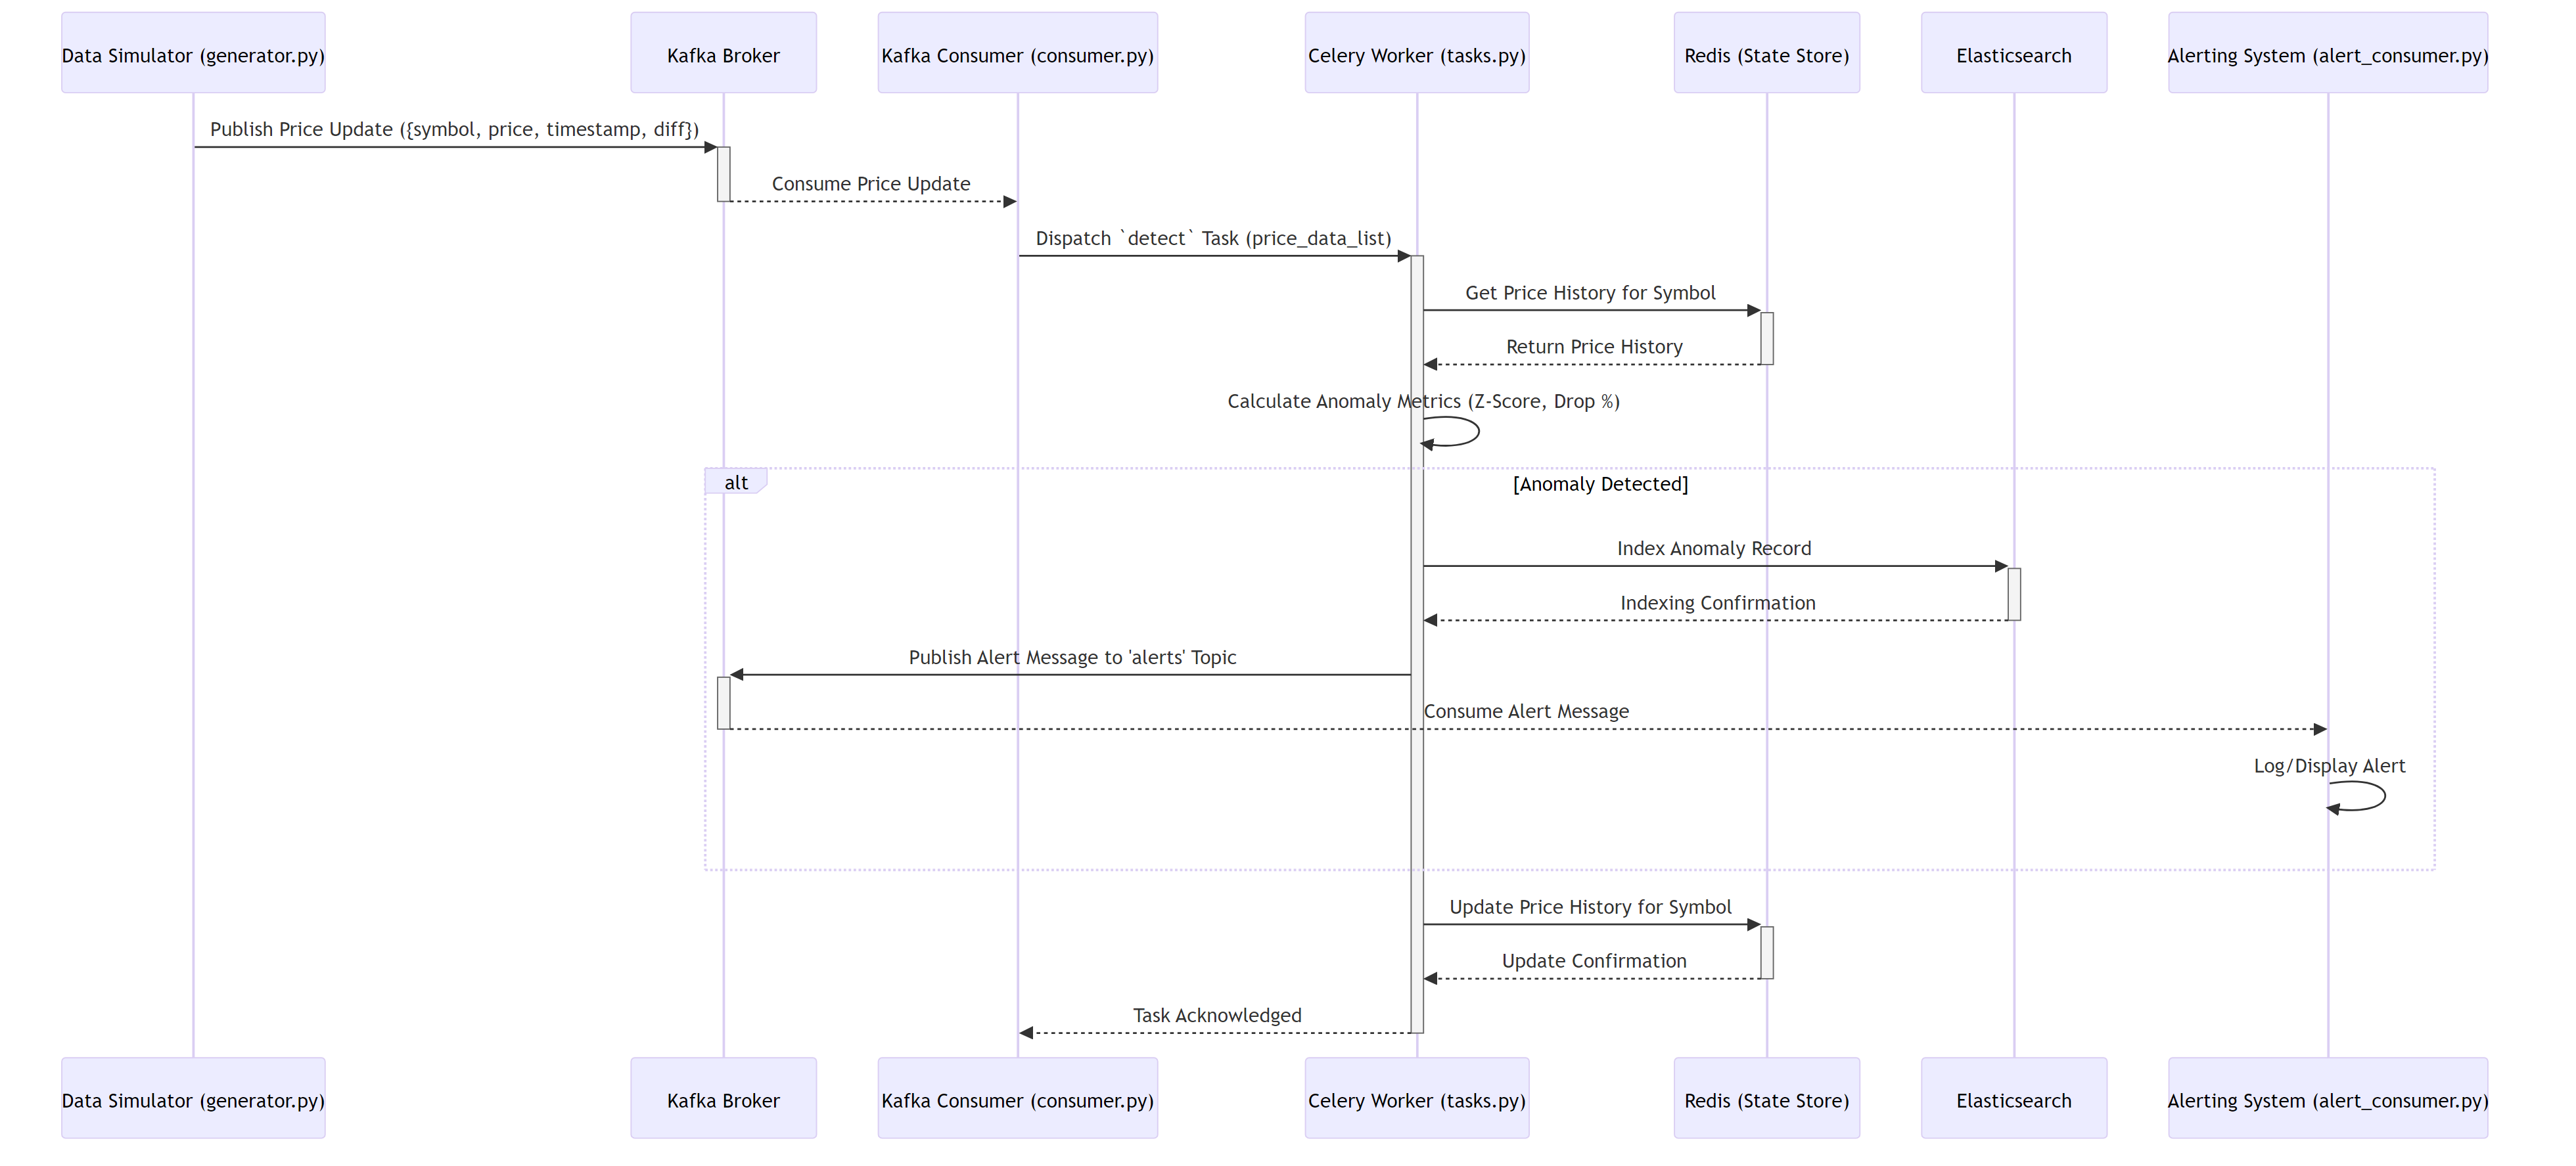
\includegraphics[width=\textwidth]{figures/backend-1.png}

\caption{A diagram showing the data flow for all the detail components described above,}

\label{fig:Expdiagram1}
\end{sidewaysfigure}

\break





\subsection{API and Reporting Layer}

\subsubsection{API Endpoints}
The Stock Anomaly Detection API provides several endpoints to fetch anomaly data and generate reports.

\paragraph{Alerting Endpoints}
\begin{itemize}
    \item \verb|GET /|: The root endpoint. Returns basic information about the API, including its name, version, and a list of available primary endpoints.
    \item \verb|GET /alerts|: Fetches all detected stock anomalies within a specified date range.
    \begin{itemize}
        \item Parameters: \verb|from| (start date), \verb|to| (end date).
    \end{itemize}
    \item \verb|GET /alerts/{symbol}/|: Retrieves anomalies for a specific stock symbol within a given date range.
    \begin{itemize}
        \item Parameters: \verb|symbol| (stock symbol), \verb|from| (start date), \verb|to| (end date).
    \end{itemize}
\end{itemize}

\paragraph{V1 Report Generation Endpoints}
The API offers robust report generation capabilities through its modern V1 endpoints, featuring powerful asynchronous operations.

\begin{itemize}
    \item \verb|POST /v1/reports|: This is the \textbf{primary endpoint} for all report-related operations. It offers a unified interface for both synchronous report generation and asynchronous generation with email delivery.
    \begin{itemize}
        \item Parameters: \verb|from|, \verb|to|, \verb|symbol|, \verb|format|.
        \item Optional Parameter: \verb|recipient_email|.
        \item \textbf{Behavior}:
        \begin{itemize}
            \item If \verb|recipient_email| is \textbf{not provided}, the report is generated synchronously and returned directly in the HTTP response.
            \item If \verb|recipient_email| \textbf{is provided}, the API gloriously initiates an \textbf{asynchronous background task} to generate the report. Upon successful completion, the report is automatically dispatched to the specified email address. This non-blocking operation allows users to continue interacting with other services or receive a quick acknowledgment (task ID) without waiting for the potentially time-consuming report generation process to finish.
        \end{itemize}
    \end{itemize}
    \item \verb|GET /v1/reports/status/{task_id}|: Allows users to check the status of an asynchronously initiated report generation task using the task ID returned by the \verb|/v1/reports| endpoint (when \verb|recipient_email| is used).
    \begin{itemize}
        \item Parameter: \verb|task_id|.
    \end{itemize}
\end{itemize}

The \verb|/v1/reports| endpoint significantly enhances user experience by providing a single, powerful interface for report generation. The asynchronous execution, particularly when coupled with email notifications, ensures that the system remains responsive and efficient, especially for large reports or during peak load times.




This next sequence diagram illustrates the interaction between the FastAPI application and the underlying data storage (Elasticsearch) and processing (Celery) for querying anomalies and generating reports.


% \subsection{Sequence Diagram: Api }

\begin{figure}[H]
    \centering
    % Placeholder for Class Diagram
    % \hspace{-3cm}
    % \includegraphics[width=0.8\textwidth]{figures/class_diagram_data_model.png}
    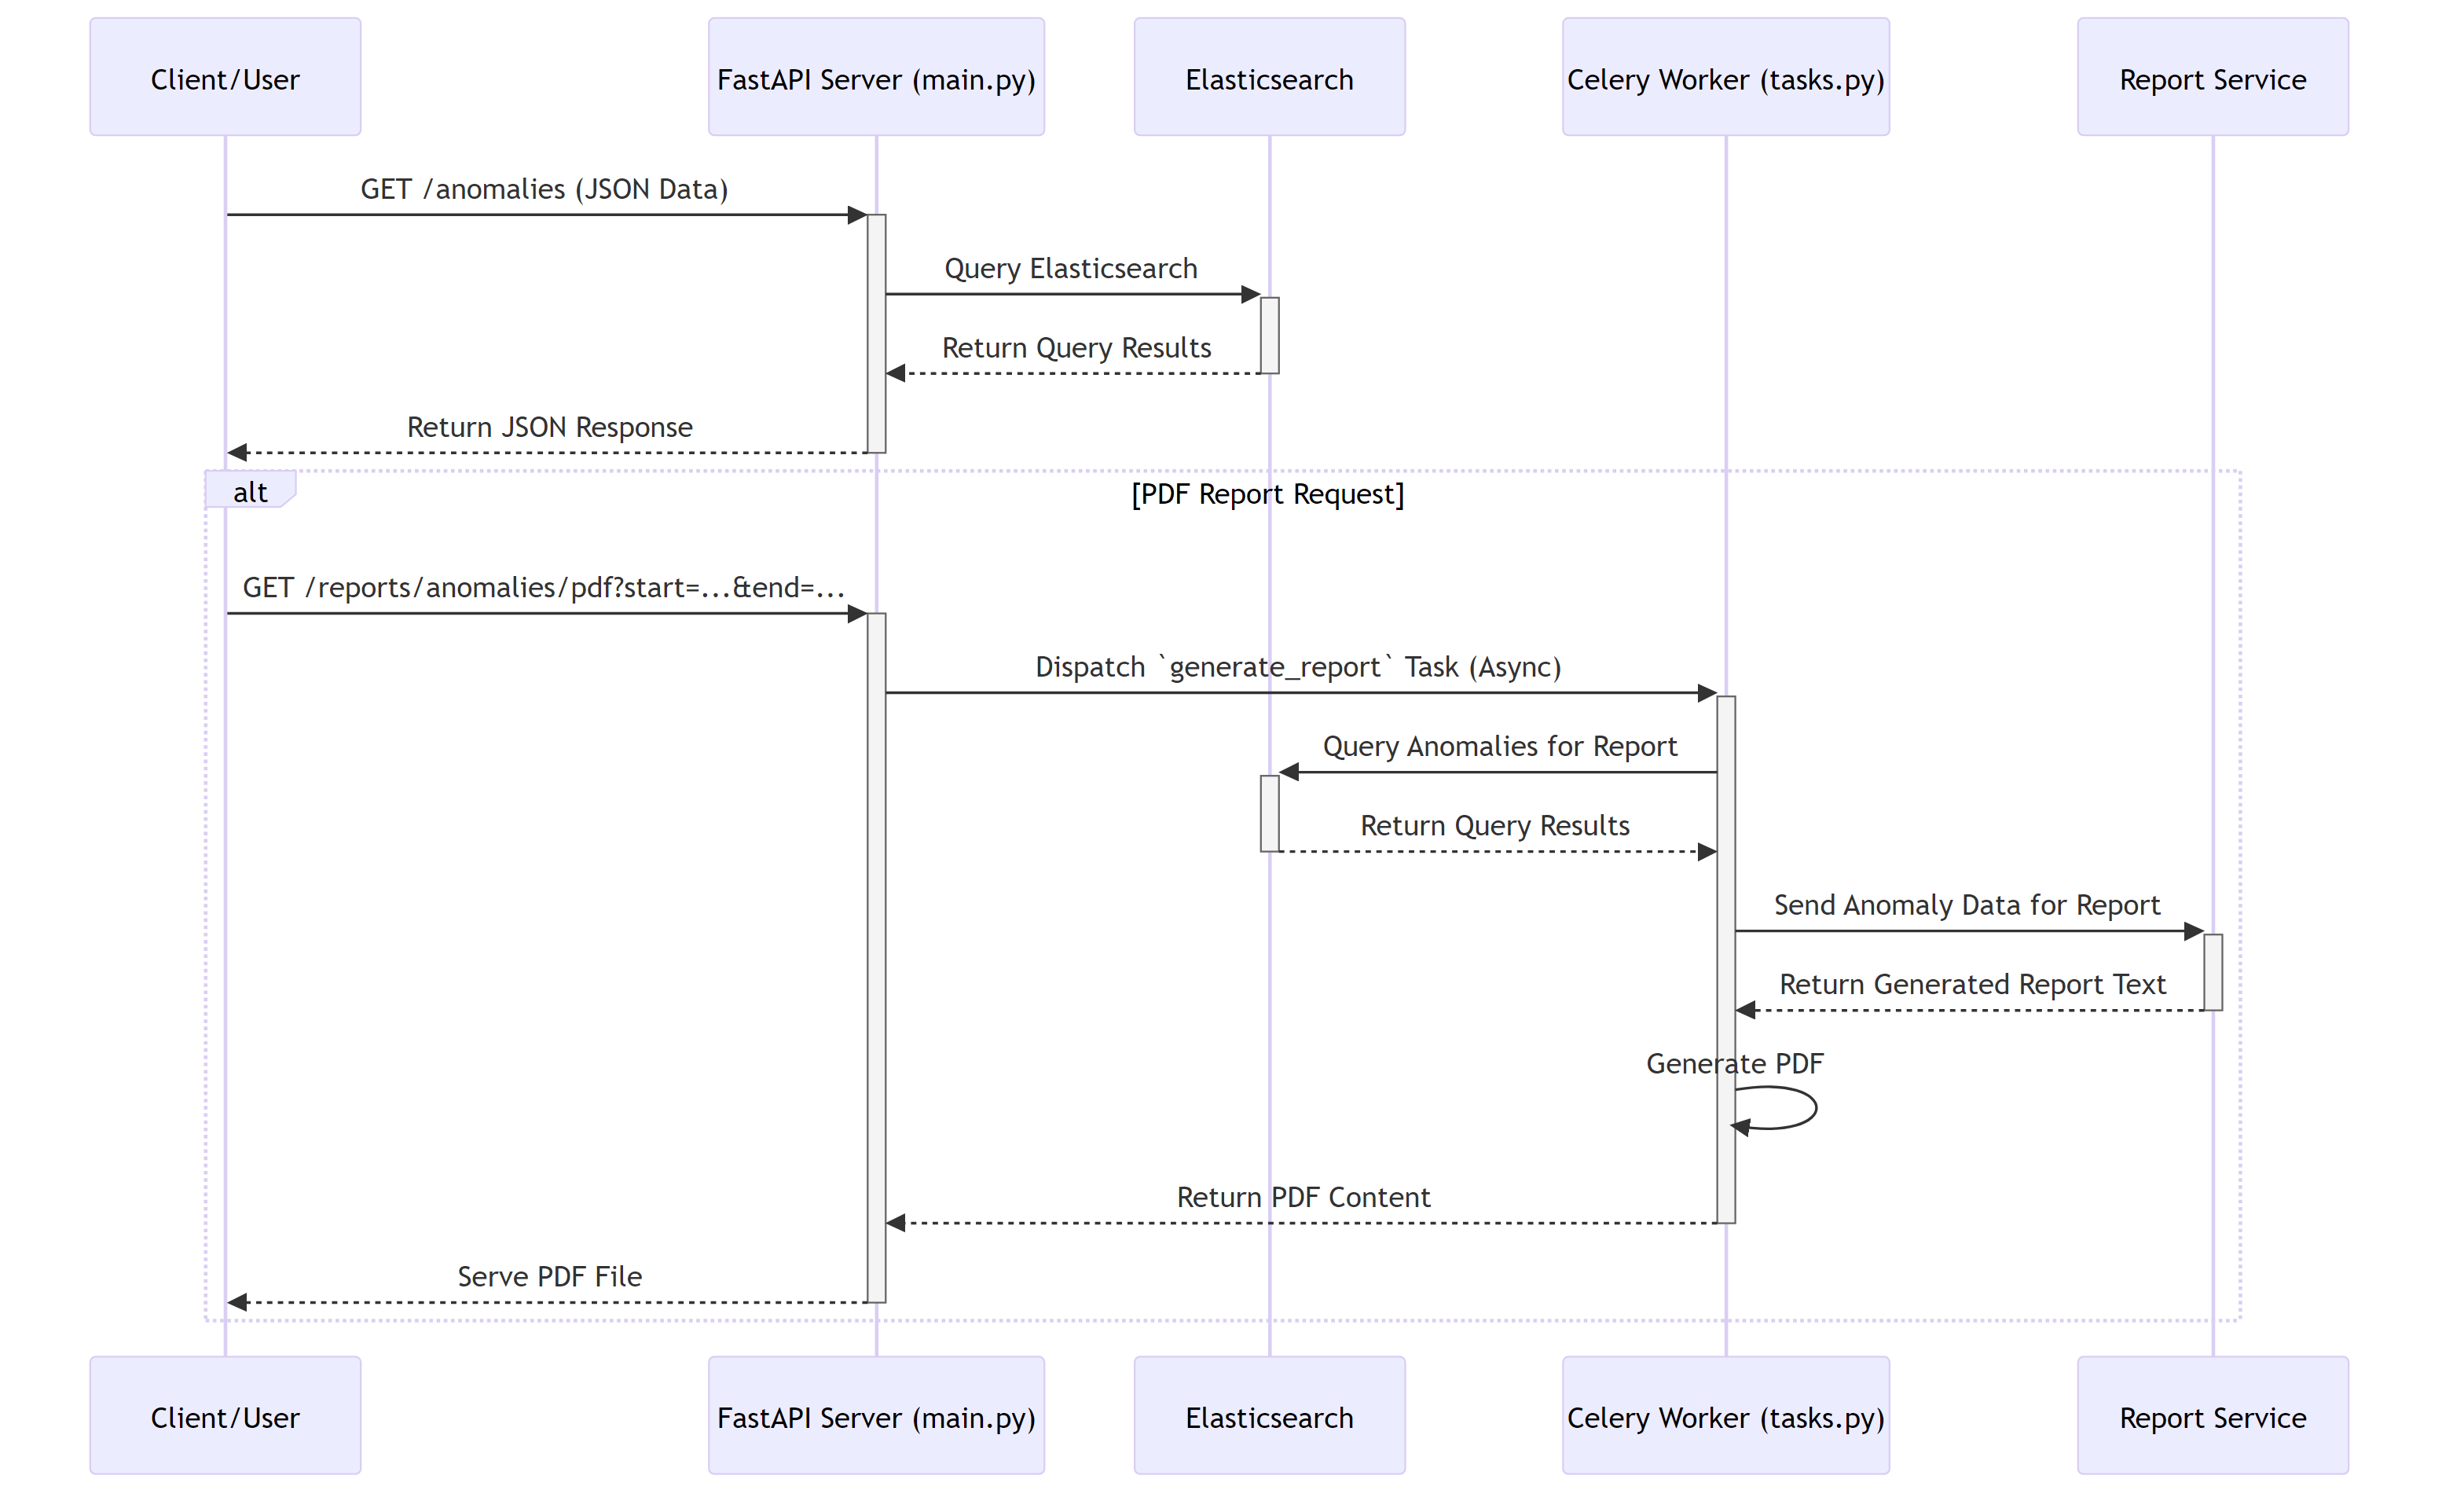
\includegraphics[width=1.2\textwidth,angle=90]{figures/api-1.png}
    \caption{Sequence Diagram for API Interactions}
    \label{fig:class_diagram_data_model}
\end{figure}

% This diagram would illustrate the sequence of interactions: FastAPI API $\rightarrow$ Elasticsearch (query anomalies) $\rightarrow$ Celery Worker (generate report) $\rightarrow$ FastAPI API (return report).
% it shows variant type of requests (geting anomalies, generating reports, etc.) and their interactions with the underlying data storage (Elasticsearch) and processing (Celery).



\subsubsection{Report Generator}

This module generates reports in multiple formats (PDF , CSV.....)
\begin{itemize}
    \item \textbf{Libraries}: e.g., `reportlab` or `WeasyPrint` for PDF, standard `csv` module for CSV.
    \item \textbf{Content}: Reports include summaries of detected anomalies, statistics, and potentially charts.
    \item \textbf{Formatting}: The formatting of the report depends on the selected format. For example, PDF reports can include sophisticated formatting with tables , enhancing readability and visual appeal. 

\begin{figure}[H]
    \centering
    \includegraphics[width=\textwidth]{figures/sad/pdf_screen.png}
    \caption{Sample PDF Report}
    \label{fig:pdf_report_screenshot}
\end{figure}

In contrast, CSV reports are formatted as comma-separated values, suitable for importing into spreadsheet software or other data analysis tools. 

\begin{figure}[H]
    \centering
    \includegraphics[width=\textwidth]{figures/sad/csv_screnn.png}
    \caption{Sample CSV Report}
    \label{fig:csv_report_screenshot}
\end{figure}
\end{itemize}

for the report generation, we use a Factory design pattern to create different report generators based on the requested format. This allows for easy extensibility if new report formats are needed in the future.
\subsection{Factory Pattern Diagram}
This diagram will illustrate the implementation of the Factory design pattern within the system, particularly for the data generation and anomaly detection modules. It will show the creator, concrete creators, product, and concrete product classes involved in the pattern.

This architecture utilizes the Factory Method design pattern, which provides an interface for creating objects in a superclass, but allows subclasses to alter the type of objects that will be created. In this specific context, the \texttt{ReportFactory} acts as the creator, abstracting the instantiation logic of different report generators (e.g., \texttt{PDFReportGenerator}, \texttt{CSVReportGenerator}).

\textbf{Why this pattern was used:}

The Factory Method pattern was chosen to decouple the client code from the concrete implementations of report generators. This means that the part of the application that needs a report doesn't need to know whether it's getting a PDF, CSV, or any other type of report. It simply requests a report generator from the \texttt{ReportFactory} based on a specified format. This promotes a clean separation of concerns and reduces direct dependencies.

\textbf{Scalability:}

This pattern significantly enhances scalability. If a new report format (e.g., Excel, XML) is required in the future, a new concrete \texttt{IReportGenerator} implementation (e.g., \texttt{ExcelReportGenerator}) can be added without modifying existing client code or the \texttt{ReportFactory}'s \texttt{get\_generator} method.

\begin{figure}[H]
    \centering
    % Placeholder for Class Diagram
    % \hspace{-3cm}
    % \includegraphics[width=0.8\textwidth]{figures/class_diagram_data_model.png}
    \includegraphics[width=\textwidth]{figures/generator-1.png}
    \caption{Factory Pattern Diagram}
    \label{fig:factory_pattern_diagram}
\end{figure}
 




\subsubsection{Alert System (Kafka Topics)}

When an anomaly is detected and confirmed, an alert message is published to a dedicated Kafka topic (e.g., \texttt{anomaly\_alerts}).
\begin{itemize}
    \item \textbf{Alert Message Format}: JSON, containing details of the anomaly and severity.
    \item \textbf{Consumers}: Separate services (not part of this core project scope but envisioned) can consume these alerts to send notifications via email, SMS, or dashboard updates.
\end{itemize}
\section{Justified Technology Choices}

\begin{itemize}
    \item \textbf{Apache Kafka}: Chosen for its high-throughput, fault-tolerant, and scalable stream processing capabilities, essential for handling real-time financial data feeds.
    
    \item \textbf{Elasticsearch}: Selected for its powerful full-text search, analytics capabilities, and horizontal scalability, making it ideal for storing, querying, and analyzing large volumes of anomaly data.
    
    \item \textbf{FastAPI (Python)}: Chosen for its high performance (comparable to NodeJS and Go), ease of use, automatic data validation with Pydantic, and built-in support for asynchronous programming, which is crucial for I/O-bound operations.
    
    \item \textbf{Celery (Python)}: Selected for distributed task processing. It allows decoupling time-consuming anomaly detection tasks from the main data ingestion flow, improving responsiveness and scalability.
    
    \item \textbf{Redis}: Chosen for its speed as an in-memory data store, perfect for managing sliding windows of recent price data required for Z-score calculations with minimal latency.
    
    \item \textbf{Python}: Used as the primary programming language due to its extensive libraries for data science (NumPy, Pandas), web development (FastAPI, Celery), and general-purpose programming, along with a large developer community.
    
    \item \textbf{Docker}: Used for containerization, ensuring consistent development, testing, and deployment environments across different machines and simplifying the management of microservices.
\end{itemize}

\section{Design Diagrams}

This section would typically include more detailed diagrams.

\subsection{Sequence Diagram: Detection Flow}


This diagram would illustrate the sequence of interactions: Data Generator $\rightarrow$ Kafka (price topic) $\rightarrow$ Celery Worker/Kafka Consumer $\rightarrow$ Redis (sliding window) $\rightarrow$ Z-Score Calculation $\rightarrow$ Elasticsearch (if anomaly) $\rightarrow$ Kafka (alert topic).

\break





\subsection{sequence Diagram: Batch report generation}
\begin{figure}[H]
    
    % Placeholder for Class Diagram
    % \hspace{-3cm}
    % \includegraphics[width=0.8\textwidth]{figures/class_diagram_data_model.png}
    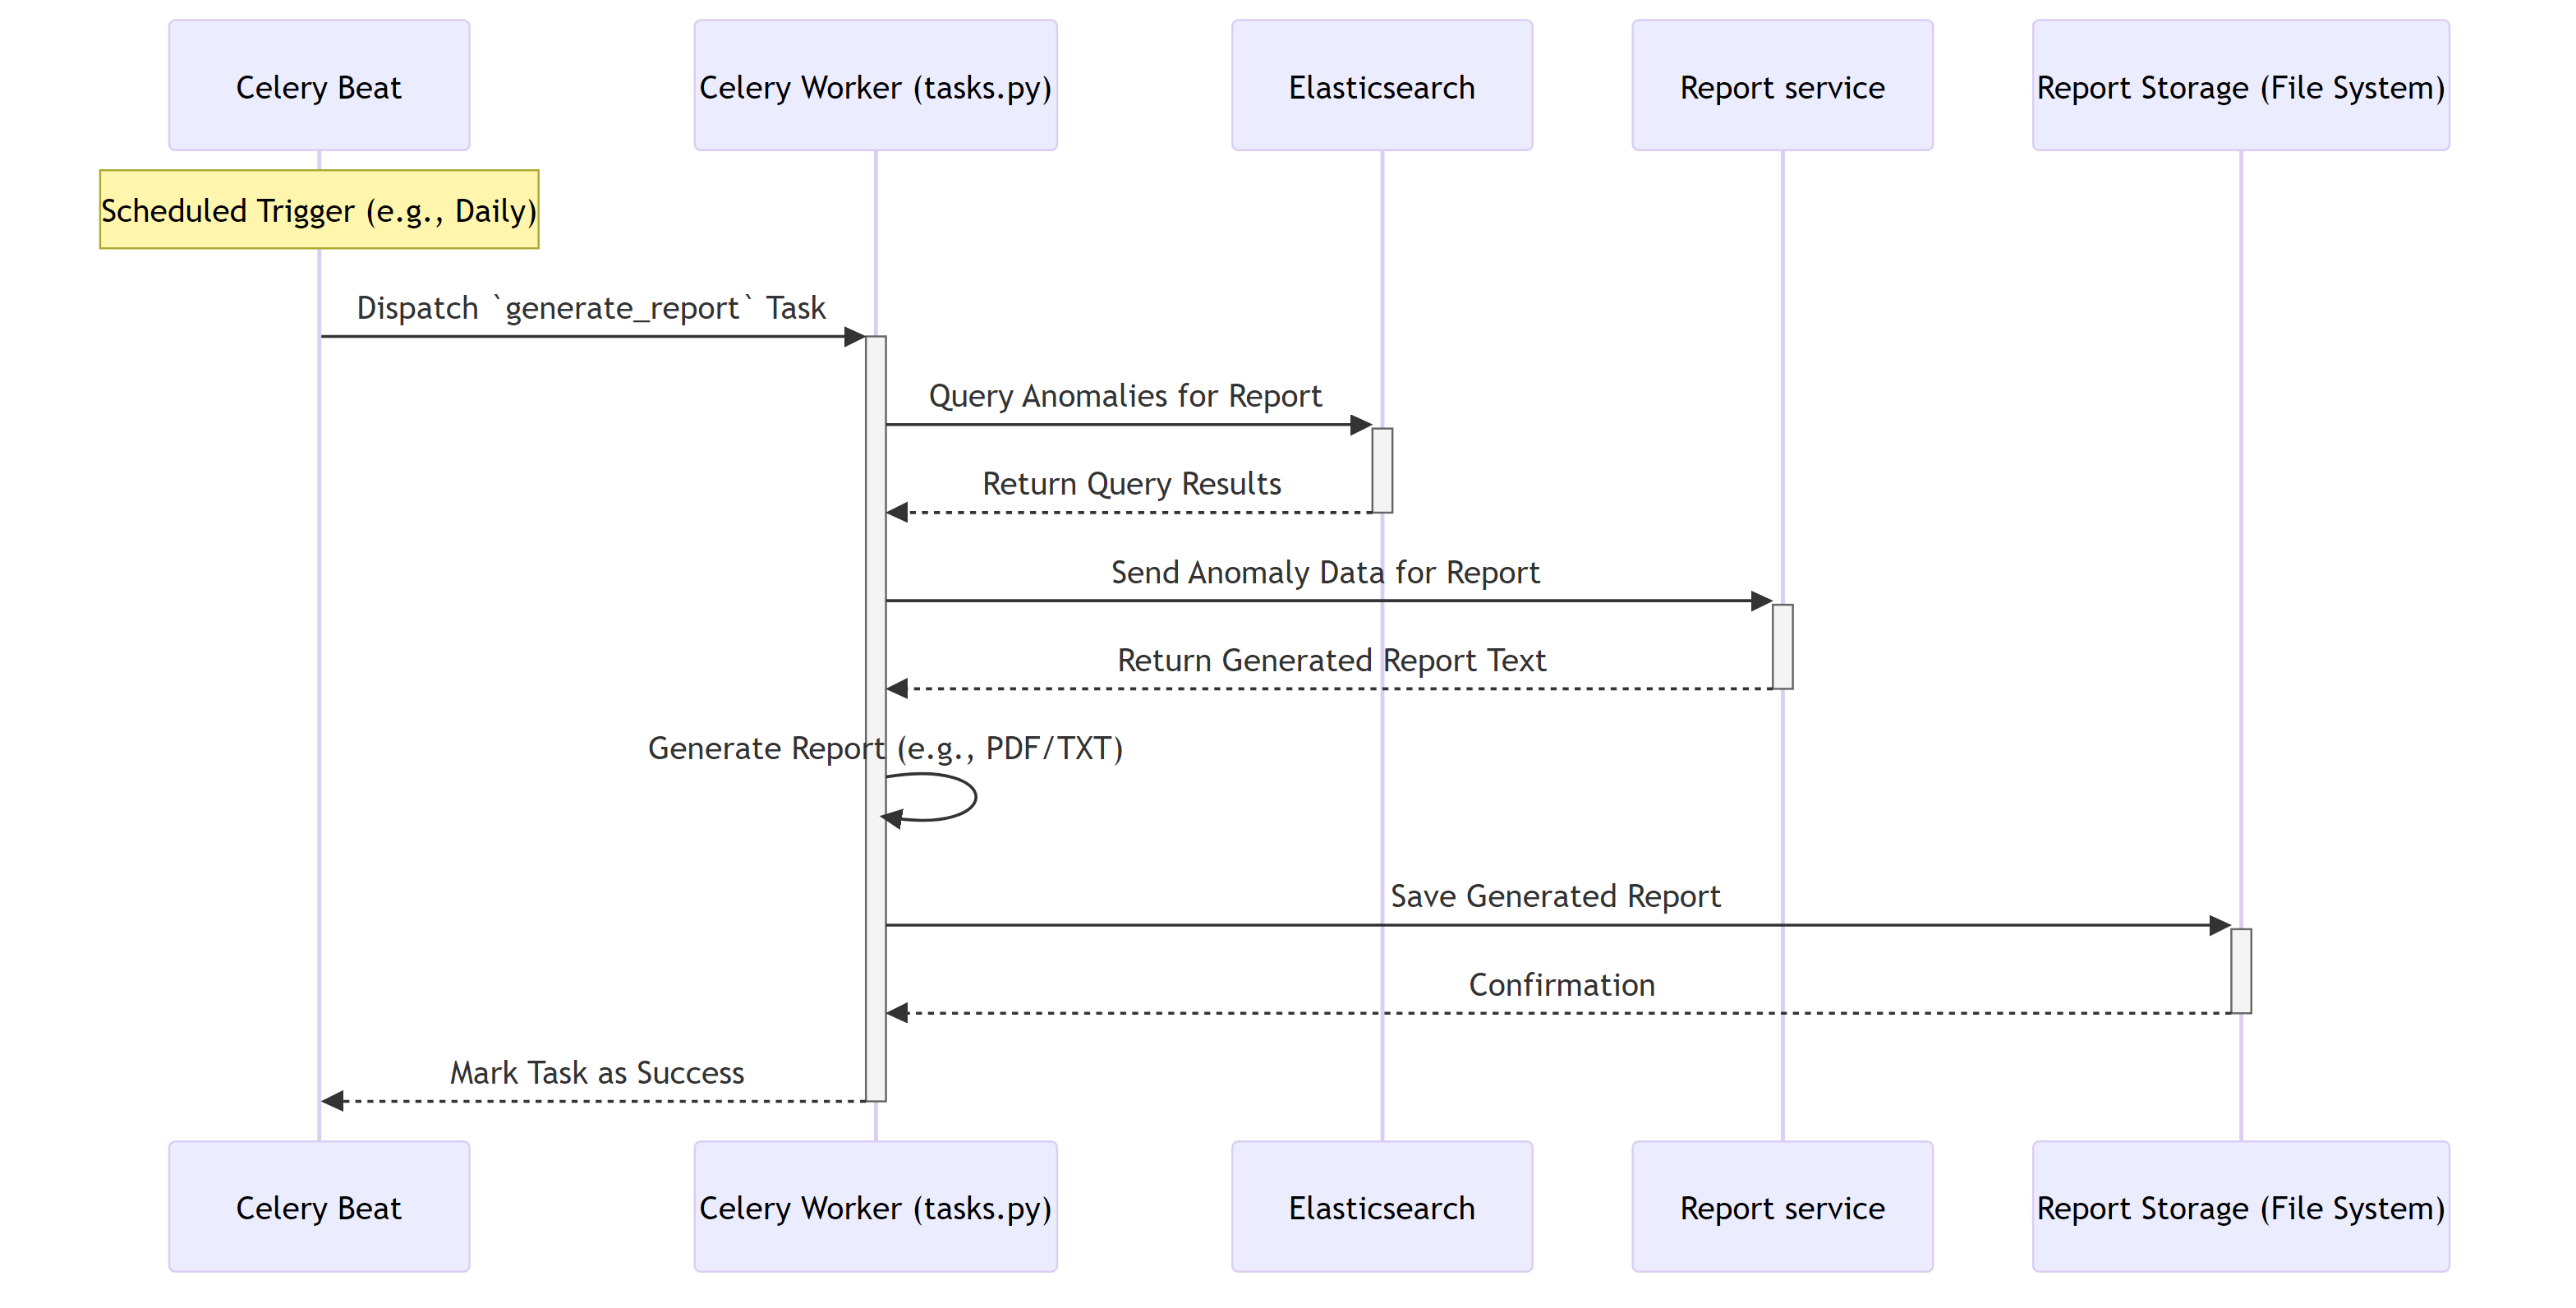
\includegraphics[width=1.2\textwidth]{figures/batch-1.png}
    \caption{Batch Report Generation Sequence Diagram}
    \label{fig:batch_report_generation_sequence_diagram}


\end{figure}


this diagram illustrate how shecduled batch report generation works, showing the interaction between the FastAPI application, Celery workers, and Elasticsearch for generating reports based on historical anomalies.
the layer responsibble for trigering the Task is the Celery Beat, which schedules the task to run at specific intervals (e.g., daily, weekly).
they work based on the linux cron system, which allows for scheduling tasks to run at specific times or intervals.

\subsection{Deployment with Docker and Docker Compose}

To orchestrate and run all the services in our architecture—Kafka, Zookeeper, Redis, Elasticsearch, and Kibana—we use Docker and Docker Compose. Docker allows us to package each service into a container, ensuring consistency across development, testing, and production environments.

\textbf{Service Ports and Networking:}
\begin{itemize}
    \item \textbf{Kafka} runs on port \texttt{9092} (for external connections) and \texttt{9093} (for internal container-to-container communication). These ports are mapped from the container to the host, allowing both local development tools and other containers to communicate with Kafka.
    \item \textbf{Zookeeper} (required by Kafka) listens on port \texttt{2181}.
    \item \textbf{Redis} runs on port \texttt{6379}. We use the \texttt{redis:7.2-alpine} image, which is based on Alpine Linux. Alpine images are chosen for their minimal size and security, reducing the attack surface and speeding up container startup.
    \item \textbf{Elasticsearch} is exposed on port \texttt{9200} for REST API access.
    \item \textbf{Kibana} is available on port \texttt{5601} for web-based visualization.
\end{itemize}

All containers are connected to a \textbf{shared Docker network} created by Docker Compose. This enables DNS-based service discovery: containers can communicate using service names (e.g., \texttt{kafka}, \texttt{redis}, \texttt{es01}) instead of IP addresses.

Docker Compose brought significant advantages to our deployment process by allowing us to define, configure, and launch all required services with a single command. It simplified service orchestration, ensured consistent environments, and made it easy to manage dependencies and networking between containers.

\begin{figure}[H]
    \centering
    \includegraphics[width=\textwidth]{figures/sad/image.png}
    \caption{Overall Docker Compose Architecture}
    \label{fig:docker_compose_architecture}
\end{figure}


This approach ensures that all services are reproducibly deployed, easily managed, and networked together, forming a robust foundation for our distributed financial data surveillance system.

% \subsection{Other UML Diagrams}
% This section provides placeholders for additional UML diagrams that can further illustrate the system's design. These diagrams will be added as the project evolves and specific design aspects require more detailed visualization.

% \subsubsection{Use Case Diagram}
% \begin{figure}[h]
%     \centering
%     \fbox{\parbox[c][6cm][c]{0.8\textwidth}{\centering Placeholder for Use Case Diagram}}
%     \caption{Placeholder for Use Case Diagram}
%     \label{fig:placeholder_use_case_diagram}
% \end{figure}

% \subsubsection{Component Diagram}
% \begin{figure}[h]
%     \centering
%     \fbox{\parbox[c][6cm][c]{0.8\textwidth}{\centering Placeholder for Component Diagram}}
%     \caption{Placeholder for Component Diagram}
%     \label{fig:placeholder_component_diagram}
% \end{figure}

% \subsubsection{Activity Diagram}
% \begin{figure}[h]
%     \centering
%     \fbox{\parbox[c][6cm][c]{0.8\textwidth}{\centering Placeholder for Activity Diagram}}
%     \caption{Placeholder for Activity Diagram}
%     \label{fig:placeholder_activity_diagram}
% \end{figure}


% % Chapter 4: Implementation
\chapter{Implementation}

\section{Development Environment}

\subsection{Technical Stack}

The project was developed using the following technical stack:
\begin{itemize}
    \item \textbf{Programming Language}: Python 3.10+
    \item \textbf{Data Streaming}: Apache Kafka 3.x
    \item \textbf{Message Broker (Celery)}: Redis 7.x (also used for sliding window)
    \item \textbf{Task Queue}: Celery 5.x
    \item \textbf{Data Storage (Anomalies)}: Elasticsearch 8.x
    \item \textbf{Web Framework (API)}: FastAPI 0.100+
    \item \textbf{Containerization}: Docker \& Docker Compose
    \item \textbf{Operating System}: Linux (Ubuntu 22.04 LTS for development and deployment)
    \item \textbf{Python Libraries}:
    \begin{itemize}
        \item \texttt{kafka-python}: For Kafka producer and consumer clients.
        \item \texttt{redis}: For interacting with Redis.
        \item \texttt{elasticsearch}: The official Elasticsearch client for Python.
        \item \texttt{celery}: For defining and running asynchronous tasks.
        \item \texttt{fastapi}: For building the REST API.
        \item \texttt{uvicorn}: ASGI server for FastAPI.
        \item \texttt{pydantic}: For data validation in FastAPI.
        \item \texttt{numpy}: For numerical operations (mean, std dev).
        \item \texttt{pandas}: (Optional) For data manipulation if needed, primarily for report generation or data loading.
        \item \texttt{reportlab} / \texttt{WeasyPrint}: For PDF report generation.
        \item \texttt{python-json-logger}: For structured logging.
    \end{itemize}
\end{itemize}

\subsection{Development Tools}
\begin{itemize}
    \item \textbf{IDE}: Visual Studio Code with Python extension, Pylance, and Docker extension.
    \item \textbf{Version Control}: Git, with a repository hosted on GitHub/GitLab.
    \item \textbf{Debugging}: VS Code debugger, Celery Flower for monitoring tasks, Kibana for Elasticsearch inspection.
    \item \textbf{API Testing}: Postman / Insomnia, or curl.
    \item \textbf{Terminal}: Linux default terminal (bash/zsh).
\end{itemize}

\subsection{Dependency Management}

Python dependencies are managed using a \texttt{requirements.txt} file. This ensures that all developers and deployment environments use the same versions of libraries, promoting consistency and reducing compatibility issues. The full list of dependencies is available in the Appendix.

Dependencies are installed using: \texttt{pip install -r requirements.txt}

\subsection{Docker for Service Containerization}

Docker and Docker Compose are used to containerize each service (Kafka, Zookeeper, Elasticsearch, Redis, FastAPI application, Celery workers, Data Generator). This approach offers:
\begin{itemize}
    \item \textbf{Environment Consistency}: Ensures services run the same way regardless of the host machine.
    \item \textbf{Isolation}: Services run in isolated environments, preventing conflicts.
    \item \textbf{Simplified Deployment}: \texttt{docker-compose up} can start the entire multi-container application.
    \item \textbf{Scalability}: Docker Swarm or Kubernetes can be used to scale services in a production environment.
\end{itemize}
A \texttt{docker-compose.yml} file defines the services, networks, and volumes. (A snippet will be shown in Chapter 6).

\section{Key Module Implementation}

\subsection{Data Generation Module}

This module simulates stock price data for TSLA and publishes it to a Kafka topic.

\subsubsection{TSLA Data Structure and Simulation}
The data generator script creates JSON objects with \texttt{symbol}, \texttt{timestamp}, \texttt{price}, and \texttt{volume}.
It simulates price movements with a baseline price and random fluctuations. Volatility can be adjusted, and artificial anomalies (sudden spikes or drops) are injected periodically to test the detection logic.

\subsubsection{Kafka Producer Integration}
The script uses the \texttt{kafka-python} library to connect to the Kafka cluster and send messages. The full implementation is available in the appendix.

\textbf{Explanations:}
\begin{itemize}
    \item The \texttt{KafkaProducer} is configured with broker addresses and a JSON serializer.
    \item A function generates data points with random fluctuations and occasional anomalies.
    \item The main loop continuously generates and sends data to the \texttt{stock\_prices} topic.
    \item Error handling and graceful shutdown of the producer are included.
\end{itemize}

\textbf{Application of Factory Design Pattern for Data Generation:}
The data generation module can leverage the Factory design pattern to create different types of data generators (e.g., for different stock symbols, or different simulation models like normal, abnormal, or stress-test data). A `DataGeneratorFactory` could provide a method to return instances of `TSLADataGenerator`, `AAPLDataGenerator`, or `CustomAnomalyGenerator` based on configuration. This promotes modularity and extensibility, allowing new data generation strategies to be added without modifying existing client code.
\begin{figure}[h!]
    \centering
    \fbox{\parbox[c][5cm][c]{0.8\textwidth}{\centering Placeholder for Data Generator Factory Pattern Diagram}}
    \caption{Placeholder for Data Generator Factory Pattern Diagram}
    \label{fig:data_generator_factory_diagram}
\end{figure}

\subsection{Detection Module (Celery Task)}

This module consumes data from Kafka and performs Z-score based anomaly detection. It runs as a Celery task.



\subsection{Storage Module (Elasticsearch Integration)}

This module is responsible for storing detected anomalies in Elasticsearch. Connection to Elasticsearch is typically managed using the official Python client. The full implementation for connection and anomaly storage is available in the appendix.

\subsubsection{Index Mapping}
The Elasticsearch index mapping (also detailed in Chapter 3) defines the structure and data types for anomaly documents. This is crucial for efficient searching and aggregation.

\subsubsection{Performance Optimizations}
\begin{itemize}
    \item \textbf{Bulk Indexing}: For high volumes, use Elasticsearch's bulk API to index multiple anomalies in a single request.
    \item \textbf{Connection Pooling}: Ensure the Elasticsearch client uses connection pooling.
    \item \textbf{Appropriate Sharding}: Configure the number of shards for the index based on expected data volume and query load.
    \item \textbf{Refresh Interval}: Adjust the index refresh interval if near real-time search is not strictly required for all use cases, to reduce indexing overhead.
\end{itemize}
 

\subsection{REST API (FastAPI)}

The FastAPI application provides endpoints for querying anomalies and generating reports.

\subsubsection{Implemented Endpoints}
Key endpoints include:
\begin{itemize}
    \item \texttt{GET /anomalies/}: Fetches anomalies, with query parameters for filtering by symbol, date range, etc.
    \item \texttt{GET /anomalies/\{anomaly\_id\}/}: Retrieves a specific anomaly by its ID.
    \texttt{POST /reports/generate/}: Initiates report generation (e.g., for a specific symbol and time range).
    \item \texttt{GET /reports/download/\{report\_id\}/}: Downloads a previously generated report.
\end{itemize}
The full implementation of these endpoints is available in the appendix.

\subsubsection{Parameter Validation}
FastAPI uses Pydantic models for automatic request and response validation, ensuring data integrity and providing clear error messages for invalid inputs.

\subsubsection{Error Handling}
Custom exception handlers and FastAPI's \texttt{HTTPException} are used to return appropriate HTTP status codes and error details to the client.

\section{Technical Challenges Encountered}

\subsection{Concurrency Management in Redis}
\begin{itemize}
    \item \textbf{Problem}: Multiple Celery workers accessing and updating Redis lists for the same symbol concurrently could lead to race conditions if not handled carefully (though Redis single-threaded operations on keys largely mitigate this for simple list operations like LPUSH/LTRIM).
    \item \textbf{Solution}: For more complex atomic operations, Redis transactions (MULTI/EXEC) or Lua scripting can be used. For this project, the atomicity of individual Redis commands (LPUSH, LTRIM, LRANGE) was generally sufficient for the sliding window logic. Distributed locks (e.g., using Redlock algorithm or a library) would be necessary if shared resources required more complex, multi-step atomic updates across different workers or services.
\end{itemize}

\subsection{Elasticsearch Query Performance}
\begin{itemize}
    \item \textbf{Problem}: As the volume of anomaly data grows, Elasticsearch queries for reports or API responses could become slow, especially with complex filters or aggregations.
    \item \textbf{Solution}:
        \begin{itemize}
            \item \textbf{Optimized Mappings}: Ensure fields used for filtering and sorting are indexed appropriately (e.g., \texttt{keyword} for exact matches, \texttt{date} for date ranges).
            \item \textbf{Targeted Queries}: Avoid \texttt{script} queries or overly broad \texttt{wildcard} queries where possible. Use \texttt{term} for exact matches and \texttt{range} for numerical/date fields.
            \item \textbf{Pagination}: Implement proper pagination for API endpoints returning large datasets.
            \item \textbf{Caching}: Consider caching frequent query results at the API layer or using Elasticsearch's query cache (though it has limitations).
            \item \textbf{Index Management}: Use time-based indices and potentially rollups for historical

\input{chapters/chapter5_testing_validation}
\input{chapters/chapter6_deployment_operations}
\input{chapters/chapter7_critical_analysis}
% Chapter 8: Conclusion
\chapter{Conclusion}

\section{Summary of Achievements}
This report presents the work completed during my internship witn LEYTON COGNITX, where I was tasked with designing and implementing a real-time financial data surveillance system. The main accomplishments of this project include:
\begin{itemize}
    \item Building a scalable, event-driven architecture based on microservices.
    \item Integrating Apache Kafka to handle high-throughput data streaming.
    \item Setting up a robust anomaly detection system using Celery and Redis.
    \item Using Elasticsearch for fast storage and retrieval of anomaly data.
    \item Developing a FastAPI-based API for querying and reporting.
    \item Containerizing all services with Docker and Docker Compose to simplify deployment.
\end{itemize}
The system is able to ingest, process, and analyze financial data in real time, detect anomalies, and provide actionable insights.

\section{Lessons Learned and Future Perspectives}

This internship with LEYTON COGNITX was a great opportunity to work on a complex distributed system and deepen my understanding of modern backend architectures, moving well beyond traditional monolithic or CRUD-based applications.

\subsection{Scalability and Complexity of Distributed Systems}
Working with microservices and distributed systems showed me how powerful and flexible they can be. Each service can be developed, deployed, and scaled independently, which is a big advantage for handling different loads in a financial context. However, I also saw firsthand that this flexibility comes with added complexity—especially when it comes to communication between services, keeping data consistent, and managing everything in production. I learned that while distributed systems are great for scaling and resilience, they require careful design and strong monitoring to keep things running smoothly. The balance between simplicity and scalability was very clear throughout the project.

\subsection{Exploring New Technologies}
This project gave me the chance to get hands-on experience with several new technologies:
\begin{itemize}
    \item \textbf{Apache Kafka}: Before this internship, I had never heard of or used Kafka. Discovering how fast, reliable, and scalable it is was a real eye-opener. I learned how major companies use Kafka for real-time data streaming, and out of curiosity about what makes it so fast, I discovered some technical details such as its custom network protocol, sequential disk writes, and the zero-copy principle with the \texttt{sendfile} syscall—all of which help explain its high performance. ,This  opened my eyes to a  new lower-level aspects of system development , which I found genuinely interesting.
    \item \textbf{API/Worker Pattern (Celery \& Redis)}: Implementing asynchronous task processing with Celery and Redis showed me how to offload heavy computations from the main API, making the system more responsive and easier to scale. This pattern is essential for building modern, scalable backend services.
    \item \textbf{Elasticsearch}: Working with Elasticsearch gave me a sense of its power as a search and analytics engine, especially for time-series data. Its near real-time indexing and strong query features are a big advantage for applications that need fast data retrieval and aggregation—much more than what traditional relational databases can offer for these use cases.
    \item \textbf{Docker \& Containerization}: Although I’d heard a lot about Docker, this was my first time using it. I learned how Docker makes it easy to set up separate containers and services, each with their own dependencies, without worrying about environment conflicts. I now see how Docker can be useful for reproducible development and deployment in many projects, not just this one.
\end{itemize}
Overall, this internship helped me discover new areas in backend development, especially in data engineering, real-time analytics, and event-driven architectures. It also reinforced the importance of choosing the right tools for building high-performance, resilient systems.

% \appendix
\chapter{Appendices}

\section{Code Snippets}

\subsection{Full Implementation Examples}

This appendix contains the full code implementations of key components that were simplified in the main report.

\subsubsection{Data Generator Complete Implementation}
The complete implementation of the data generator module, including simulation logic and Kafka producer integration, is available in the project's GitHub repository.

\subsubsection{Docker Compose Configuration}
\begin{minted}[fontsize=\footnotesize, frame=lines, label=Docker Compose Configuration]{yaml}
# docker-compose.yml
version: '3.8'

services:
  # Kafka and Zookeeper
  zookeeper:
    image: confluentinc/cp-zookeeper:7.3.0
    hostname: zookeeper
    container_name: zookeeper
    ports:
      - "2181:2181"
    environment:
      ZOOKEEPER_CLIENT_PORT: 2181
      ZOOKEEPER_TICK_TIME: 2000
    volumes:
      - zookeeper-data:/var/lib/zookeeper/data
      - zookeeper-log:/var/lib/zookeeper/log

  kafka:
    image: confluentinc/cp-kafka:7.3.0
    hostname: kafka
    container_name: kafka
    depends_on:
      - zookeeper
    ports:
      - "9092:9092"
      - "29092:29092"
    environment:
      KAFKA_BROKER_ID: 1
      KAFKA_ZOOKEEPER_CONNECT: zookeeper:2181
      KAFKA_ADVERTISED_LISTENERS: PLAINTEXT://kafka:9092,PLAINTEXT_HOST://localhost:29092
      KAFKA_LISTENER_SECURITY_PROTOCOL_MAP: PLAINTEXT:PLAINTEXT,PLAINTEXT_HOST:PLAINTEXT
      KAFKA_INTER_BROKER_LISTENER_NAME: PLAINTEXT
      KAFKA_OFFSETS_TOPIC_REPLICATION_FACTOR: 1
      KAFKA_LOG_RETENTION_HOURS: 24
    volumes:
      - kafka-data:/var/lib/kafka/data

  # Redis (for Celery broker and sliding window)
  redis:
    image: redis:7-alpine
    container_name: redis
    ports:
      - "6379:6379"
    command: redis-server --appendonly yes
    volumes:
      - redis-data:/data

  # Elasticsearch
  elasticsearch:
    image: docker.elastic.co/elasticsearch/elasticsearch:8.7.0
    container_name: elasticsearch
    environment:
      - discovery.type=single-node
      - ES_JAVA_OPTS=-Xms512m -Xmx512m
      - xpack.security.enabled=false
    ports:
      - "9200:9200"
    volumes:
      - es-data:/usr/share/elasticsearch/data

  # FastAPI application
  api:
    build:
      context: ./api
      dockerfile: Dockerfile
    container_name: financial-api
    ports:
      - "8000:8000"
    depends_on:
      - kafka
      - redis
      - elasticsearch
    environment:
      - KAFKA_BROKERS=kafka:9092
      - REDIS_HOST=redis
      - ELASTICSEARCH_HOST=elasticsearch
      - ELASTICSEARCH_PORT=9200
    volumes:
      - ./api:/app

  # Celery workers
  worker:
    build:
      context: ./worker
      dockerfile: Dockerfile
    container_name: celery-worker
    depends_on:
      - kafka
      - redis
      - elasticsearch
    environment:
      - KAFKA_BROKERS=kafka:9092
      - REDIS_HOST=redis
      - ELASTICSEARCH_HOST=elasticsearch
      - ELASTICSEARCH_PORT=9200
    volumes:
      - ./worker:/app

  # Data generator
  data-generator:
    build:
      context: ./data_generator
      dockerfile: Dockerfile
    container_name: data-generator
    depends_on:
      - kafka
    environment:
      - KAFKA_BROKERS=kafka:9092
    volumes:
      - ./data_generator:/app

volumes:
  zookeeper-data:
  zookeeper-log:
  kafka-data:
  redis-data:
  es-data:
\end{minted}

\section{Project Structure}
\begin{minted}[fontsize=\footnotesize, frame=lines, label=Project Structure]{text}
financial-data-surveillance-system/
|-- api/
|   |-- app/
|   |   |-- __init__.py
|   |   |-- main.py              # FastAPI application
|   |   |-- routes/              # API routes
|   |   |-- models/              # Pydantic models
|   |   |-- services/            # Business logic
|   |   `-- utils/               # Utility functions
|   |-- Dockerfile
|   `-- requirements.txt
|
|-- data_generator/
|   |-- generator.py             # Stock price simulator
|   |-- Dockerfile
|   `-- requirements.txt
|
|-- worker/
|   |-- tasks.py                 # Celery tasks
|   |-- anomaly_detection.py     # Anomaly detection algorithms
|   |-- Dockerfile
|   `-- requirements.txt
|
|-- docker-compose.yml           # Docker Compose configuration
|
|-- docs/
|   `-- api.yaml                 # OpenAPI specification
|
`-- README.md
\end{minted}

\section{Detailed Configuration Files}

\subsection{Celery Configuration}
The detailed Celery configuration, including broker and backend settings, task serialization, and Redis/Elasticsearch client initialization, is available in the project's source code.
`'

\end{document}
